
\documentclass{optica-article}
\journal{opticajournal}
\articletype{Research Article}
\usepackage{amsmath}
% AUTO-GENERATED by scripts/make_numbers_tex.py -- DO NOT HAND-EDIT.
% Regenerate: python scripts/make_numbers_tex.py
\usepackage{xcolor}  % for the [PENDING] flag color, harmless if already loaded

\newcommand{\MeasuredContrastTwoX}{2.00}
\newcommand{\KcPredTwoX}{4.22}
\newcommand{\KstarTwoXInterp}{4.18}
\newcommand{\KstarTwoXCI}{\textcolor{red}{[PENDING]}}
\newcommand{\MeanGainTwoX}{0.40}
\newcommand{\MinGainTwoX}{-0.03}
\newcommand{\MeasuredContrastFourX}{3.80}
\newcommand{\KcPredFourX}{6.96}
\newcommand{\KstarFourXInterp}{\textcolor{red}{[PENDING]}}
\newcommand{\KstarFourXCI}{8.98}
\newcommand{\MeanGainFourX}{0.70}
\newcommand{\MinGainFourX}{0.04}
\newcommand{\MeasuredContrastEightX}{5.32}
\newcommand{\KcPredEightX}{9.33}
\newcommand{\KstarEightXInterp}{\textcolor{red}{[PENDING]}}
\newcommand{\KstarEightXCI}{8.98}
\newcommand{\MeanGainEightX}{0.88}
\newcommand{\MinGainEightX}{0.05}
\newcommand{\MinGainAllBudgets}{-0.03}
\newcommand{\SEightGainKLowSlantZero}{0.913}
\newcommand{\SEightLoKLowSlantZero}{0.906}
\newcommand{\SEightHiKLowSlantZero}{0.920}
\newcommand{\SEightGainKLowSlantTwoFive}{3.122}
\newcommand{\SEightLoKLowSlantTwoFive}{3.122}
\newcommand{\SEightHiKLowSlantTwoFive}{3.123}
\newcommand{\SEightGainKLowSlantFive}{2.077}
\newcommand{\SEightLoKLowSlantFive}{2.076}
\newcommand{\SEightHiKLowSlantFive}{2.078}
\newcommand{\SEightGainKLowSlantSevenFive}{0.227}
\newcommand{\SEightLoKLowSlantSevenFive}{0.223}
\newcommand{\SEightHiKLowSlantSevenFive}{0.230}
\newcommand{\SEightGainKLowSlantTen}{0.089}
\newcommand{\SEightLoKLowSlantTen}{0.089}
\newcommand{\SEightHiKLowSlantTen}{0.089}
\newcommand{\SEightGainKLowSlantFifteen}{-0.007}
\newcommand{\SEightLoKLowSlantFifteen}{-0.016}
\newcommand{\SEightHiKLowSlantFifteen}{0.002}
\newcommand{\SEightGainKLowSlantTwenty}{0.024}
\newcommand{\SEightLoKLowSlantTwenty}{0.019}
\newcommand{\SEightHiKLowSlantTwenty}{0.028}
\newcommand{\SEightGainKMidSlantZero}{0.899}
\newcommand{\SEightLoKMidSlantZero}{0.898}
\newcommand{\SEightHiKMidSlantZero}{0.901}
\newcommand{\SEightGainKMidSlantTwoFive}{1.017}
\newcommand{\SEightLoKMidSlantTwoFive}{0.980}
\newcommand{\SEightHiKMidSlantTwoFive}{1.055}
\newcommand{\SEightGainKMidSlantFive}{2.045}
\newcommand{\SEightLoKMidSlantFive}{2.044}
\newcommand{\SEightHiKMidSlantFive}{2.046}
\newcommand{\SEightGainKMidSlantSevenFive}{0.291}
\newcommand{\SEightLoKMidSlantSevenFive}{0.210}
\newcommand{\SEightHiKMidSlantSevenFive}{0.371}
\newcommand{\SEightGainKMidSlantTen}{0.185}
\newcommand{\SEightLoKMidSlantTen}{0.182}
\newcommand{\SEightHiKMidSlantTen}{0.187}
\newcommand{\SEightGainKMidSlantFifteen}{0.046}
\newcommand{\SEightLoKMidSlantFifteen}{0.045}
\newcommand{\SEightHiKMidSlantFifteen}{0.046}
\newcommand{\SEightGainKMidSlantTwenty}{0.011}
\newcommand{\SEightLoKMidSlantTwenty}{0.011}
\newcommand{\SEightHiKMidSlantTwenty}{0.011}
\newcommand{\NZZeroPooledGainThirtyTwo}{0.640}
\newcommand{\NZZeroPooledLoThirtyTwo}{0.640}
\newcommand{\NZZeroPooledHiThirtyTwo}{0.640}
\newcommand{\NZZeroPooledGainOneTwentyEight}{0.641}
\newcommand{\NZZeroPooledLoOneTwentyEight}{0.641}
\newcommand{\NZZeroPooledHiOneTwentyEight}{0.641}
\newcommand{\NZZeroPooledGainTwoFiftySix}{0.645}
\newcommand{\NZZeroPooledLoTwoFiftySix}{0.645}
\newcommand{\NZZeroPooledHiTwoFiftySix}{0.645}
\newcommand{\NZZeroGainKLowThirtyTwo}{1.019}
\newcommand{\NZZeroGainKLowOneTwentyEight}{0.915}
\newcommand{\NZZeroGainKLowTwoFiftySix}{0.894}
\newcommand{\NZZeroGainKMidThirtyTwo}{0.731}
\newcommand{\NZZeroGainKMidOneTwentyEight}{0.900}
\newcommand{\NZZeroGainKMidTwoFiftySix}{0.928}
\newcommand{\SOneBaselineGain}{1.81}
\newcommand{\SOneNoSaturationGain}{2.22}
\newcommand{\SOneNoSaturationRatio}{1.2}
\newcommand{\SOneNoDiffusionRatio}{1.14}
\newcommand{\SOneNoNonlocalityRatio}{0.98}
\newcommand{\SOneNoDyeDepletionRatio}{0.98}
\newcommand{\STwoBaselineGain}{0.11}
\newcommand{\STwoGainMin}{0.08}
\newcommand{\STwoGainMax}{0.15}
\newcommand{\SThreeNominalGain}{1.81}
\newcommand{\SThreeWorstWithinFifty}{1.17}
\newcommand{\SThreeWorstWithinFiftyParam}{dn\_max}
\newcommand{\SThreeBestWithinFifty}{1.92}
\newcommand{\SThreeDnMaxFlipPct}{473}
\newcommand{\SThreeDnMaxWorstGain}{-3.73}
\newcommand{\SThreeDnMaxAtHundred}{0.99}
\newcommand{\SThreeDnMaxMostNegativePct}{-83}
\newcommand{\SThreeDnMaxAtMostNegative}{0.38}
\newcommand{\SThreeDnMaxMostPositivePct}{473}
\newcommand{\SThreeDnMaxAtMostPositive}{-3.73}
\newcommand{\SThreeAnyFlipWithinFifty}{no}
\newcommand{\SATMeanGainTwoX}{0.07}
\newcommand{\SATFracOfMILTwoX}{18}
\newcommand{\SATMeanGainFourX}{0.20}
\newcommand{\SATFracOfMILFourX}{28}
\newcommand{\SATMeanGainEightX}{0.36}
\newcommand{\SATFracOfMILEightX}{42}
\newcommand{\SATFitNRMSE}{0.103}
\newcommand{\SATFitAEff}{7.05}
\newcommand{\SATSubCliffGain}{0.98}
\newcommand{\SATSubCliffMILGain}{1.37}
\newcommand{\SATSubCliffFracOfMIL}{71}
\newcommand{\SATSubCliffFracMin}{79}
\newcommand{\SATSubCliffFracMax}{79}
\newcommand{\SATSubCliffK}{1.31}
\newcommand{\SATNearCliffK}{3.93}
\newcommand{\SATNearCliffFrac}{56}
\newcommand{\SATPostCliffK}{5.24}
\newcommand{\SATPostCliffFracMin}{-28}
\newcommand{\SATPostCliffFracMax}{-28}
\newcommand{\SeedCountMin}{3}
\newcommand{\SeedCountMax}{3}
\newcommand{\SeedCountDesc}{3}
\newcommand{\SeedCountModal}{3}
\newcommand{\SeedCountNExtraConfigs}{0}
\newcommand{\SeedCount}{3}
\newcommand{\NResultFiles}{2375}

% --- supplement macros (already-real data, not Phase-3-gated) ---
\newcommand{\AblationCheckpointCosSim}{1.000}
\newcommand{\AblationSurrogateCosSim}{0.844}
\newcommand{\RCWAMaxDevThreeCase}{0.038}
\newcommand{\RCWAVGridMaxDev}{0.980}
\newcommand{\RCWAVGridNCases}{90}
\newcommand{\RCWAUnslantedMaxDev}{0.29}
\newcommand{\RCWANormalMedianDev}{0.001}
\newcommand{\MeshPSNRSpread}{0.036}
\newcommand{\WavelengthDesignPSNR}{6.63}

% --- validation (Phase 6 / Section 6) macros ---
\newcommand{\NLiteratureSources}{3}
\newcommand{\NRMSEBruderGrowthDnKExp}{0.28}
\newcommand{\NRMSEBruderGrowthDnKSim}{0.17}
\newcommand{\NRMSEHsiehGrowthDnK}{0.10}
\newcommand{\NRMSEWorstFit}{0.28}
\newcommand{\NRMSEBestFit}{0.10}
\newcommand{\NGoodFits}{3}
\newcommand{\NRMSEWorstInRegime}{0.28}
\newcommand{\NRMSEBestInRegime}{0.17}
\newcommand{\NInRegimeSources}{2}
\newcommand{\BayfolDnMaxRatio}{5.7}

% --- baseline completeness (Sec. 5.2 / F4b) macros ---
\newcommand{\GSGainMin}{-1.27}
\newcommand{\GSGainMax}{0.00}
\newcommand{\LPCGainMin}{-1.82}
\newcommand{\LPCGainMax}{0.07}
\newcommand{\MILGainMinAtTwoX}{-0.03}

% --- shrinkage-induced shift bound (Discussion) macros ---
\newcommand{\ShrinkagePct}{0.5}
\newcommand{\ShrinkageSlantDeg}{20}
\newcommand{\ShrinkageThicknessUm}{30}
\newcommand{\ShrinkageShiftNm}{54.6}
\newcommand{\ShrinkageFracLowK}{1.7}
\newcommand{\ShrinkageFracHighK}{13.7}

% --- cost-benefit (Sec. 5.1) macros ---
\newcommand{\ComputeMatchRatio}{21.7}

% --- R1 reconstruction figure macros ---
\newcommand{\ROneSeedValue}{0}

% --- WP3 baseline (RSGD/GPC, Sec. 5.2) macros ---
\newcommand{\RSGDGainMin}{-0.00}
\newcommand{\RSGDGainMax}{0.00}
\newcommand{\GPCGainMin}{-1.98}
\newcommand{\GPCGainMax}{0.07}
\newcommand{\GPCLPCMaxAbsDiffTwoX}{0.18}

% --- WP4 (target ensemble / noise robustness, Sec. 5.x) macros ---
\newcommand{\SFourGainBarsTwoX}{0.90}
\newcommand{\SFourBootCILoBarsTwoX}{0.90}
\newcommand{\SFourBootCIHiBarsTwoX}{0.90}
\newcommand{\SFourGainBarsEightX}{1.95}
\newcommand{\SFourBootCILoBarsEightX}{1.95}
\newcommand{\SFourBootCIHiBarsEightX}{1.95}
\newcommand{\SFourGainSpotsTwoX}{3.22}
\newcommand{\SFourBootCILoSpotsTwoX}{3.19}
\newcommand{\SFourBootCIHiSpotsTwoX}{3.23}
\newcommand{\SFourGainSpotsEightX}{4.07}
\newcommand{\SFourBootCILoSpotsEightX}{3.99}
\newcommand{\SFourBootCIHiSpotsEightX}{4.12}
\newcommand{\SFourGainRandomBinaryTwoX}{0.17}
\newcommand{\SFourBootCILoRandomBinaryTwoX}{0.17}
\newcommand{\SFourBootCIHiRandomBinaryTwoX}{0.17}
\newcommand{\SFourGainRandomBinaryEightX}{0.24}
\newcommand{\SFourBootCILoRandomBinaryEightX}{0.24}
\newcommand{\SFourBootCIHiRandomBinaryEightX}{0.24}
\newcommand{\SFiveNoiseStdPct}{5}
\newcommand{\SFiveNoiselessGain}{0.90}
\newcommand{\SFiveNoisyGain}{0.88}

% --- WP5 (joint miscalibration Monte Carlo, Sec. 5.x) macros ---
\newcommand{\SSixNDraws}{30}
\newcommand{\SSixMeanGain}{1.76}
\newcommand{\SSixBootCILo}{1.73}
\newcommand{\SSixBootCIHi}{1.79}
\newcommand{\SSixNNegative}{0}
\newcommand{\SSixWorstDrawGain}{1.61}
\newcommand{\SSixBestDrawGain}{1.94}
\newcommand{\SSixPctRange}{25}

% --- WP6 (depth-resolved absorption, Sec. 5.x) macros ---
\newcommand{\SSevenGainODZero}{1.81}
\newcommand{\SSevenGainODOneTenth}{1.51}
\newcommand{\SSevenGainODThreeTenths}{1.45}

% --- PATH_TO_7 rewrite macros (complete M1 cells only) ---
\newcommand{\MOneNK}{10}
\newcommand{\MOneNCells}{30}
\newcommand{\MOneKMin}{1.96}
\newcommand{\MOneKMax}{15.71}
\newcommand{\MOneKList}{1.96, 2.62, 3.49, 3.93, 4.19, 4.83, 5.71, 6.98, 8.98, 15.71}
\newcommand{\MOneNPositive}{29}
\newcommand{\MOneNCIAboveZero}{27}
\newcommand{\MOneNCIIncludesZero}{2}
\newcommand{\MOneNNegative}{1}
\newcommand{\MOneNegK}{4.19}
\newcommand{\MOneNegBudget}{2}
\newcommand{\MOneNegGain}{-0.03}
\newcommand{\MOneNegCILo}{-0.05}
\newcommand{\MOneNegCIHi}{-0.005}
\newcommand{\MaxGainTwoX}{1.42}
\newcommand{\MaxGainKTwoX}{2.62}
\newcommand{\GainHighKTwoX}{0.01}
\newcommand{\GainHighKLoTwoX}{0.002}
\newcommand{\GainHighKHiTwoX}{0.008}
\newcommand{\MaxGainFourX}{2.13}
\newcommand{\MaxGainKFourX}{1.96}
\newcommand{\GainHighKFourX}{0.04}
\newcommand{\GainHighKLoFourX}{0.009}
\newcommand{\GainHighKHiFourX}{0.062}
\newcommand{\MaxGainEightX}{2.52}
\newcommand{\MaxGainKEightX}{2.62}
\newcommand{\GainHighKEightX}{0.05}
\newcommand{\GainHighKLoEightX}{0.019}
\newcommand{\GainHighKHiEightX}{0.091}
\newcommand{\MOneNExcluded}{0}
\newcommand{\SOneGBaselineSub}{4.41}
\newcommand{\SOneGBaselineNear}{0.90}
\newcommand{\SOneGBaselinePost}{0.11}
\newcommand{\SOneGNoSatSub}{5.39}
\newcommand{\SOneGNoSatNear}{0.61}
\newcommand{\SOneGNoSatPost}{0.66}
\newcommand{\SOneGNoDiffSub}{4.93}
\newcommand{\SOneGNoDiffNear}{1.14}
\newcommand{\SOneGNoDiffPost}{0.10}
\newcommand{\SOneGNoNonlocSub}{4.47}
\newcommand{\SOneGNoNonlocNear}{0.82}
\newcommand{\SOneGNoNonlocPost}{0.05}
\newcommand{\SOneGNoDyeSub}{4.36}
\newcommand{\SOneGNoDyeNear}{0.84}
\newcommand{\SOneGNoDyePost}{0.11}
\newcommand{\SOneKSub}{1.31}
\newcommand{\SOneKNear}{3.93}
\newcommand{\SOneKPost}{5.24}
\newcommand{\SXGBaselineSub}{4.41}
\newcommand{\SXNBaselineSub}{3}
\newcommand{\SXGBaselineNear}{0.90}
\newcommand{\SXNBaselineNear}{3}
\newcommand{\SXGBaselinePost}{0.11}
\newcommand{\SXNBaselinePost}{3}
\newcommand{\SXGNoMonomerSub}{-0.12}
\newcommand{\SXNNoMonomerSub}{3}
\newcommand{\SXGNoMonomerNear}{-0.09}
\newcommand{\SXNNoMonomerNear}{3}
\newcommand{\SXGNoMonomerPost}{-0.08}
\newcommand{\SXNNoMonomerPost}{3}
\newcommand{\SXGNoDyeSub}{4.35}
\newcommand{\SXNNoDyeSub}{3}
\newcommand{\SXGNoDyeNear}{0.84}
\newcommand{\SXNNoDyeNear}{3}
\newcommand{\SXGNoDyePost}{0.11}
\newcommand{\SXNNoDyePost}{3}
\newcommand{\SXGNoSatSub}{5.38}
\newcommand{\SXNNoSatSub}{3}
\newcommand{\SXGNoSatNear}{0.62}
\newcommand{\SXNNoSatNear}{3}
\newcommand{\SXGNoSatPost}{0.66}
\newcommand{\SXNNoSatPost}{3}
\newcommand{\SXGOnlyTanhSub}{-0.10}
\newcommand{\SXNOnlyTanhSub}{3}
\newcommand{\SXGOnlyTanhNear}{-0.02}
\newcommand{\SXNOnlyTanhNear}{3}
\newcommand{\SXGOnlyTanhPost}{-0.03}
\newcommand{\SXNOnlyTanhPost}{3}
\newcommand{\SXGOnlyDyeSub}{14.37}
\newcommand{\SXNOnlyDyeSub}{3}
\newcommand{\SXGOnlyDyeNear}{6.38}
\newcommand{\SXNOnlyDyeNear}{3}
\newcommand{\SXGOnlyDyePost}{7.40}
\newcommand{\SXNOnlyDyePost}{3}
\newcommand{\SXGOnlyMonomerSub}{5.75}
\newcommand{\SXNOnlyMonomerSub}{3}
\newcommand{\SXGOnlyMonomerNear}{1.73}
\newcommand{\SXNOnlyMonomerNear}{3}
\newcommand{\SXGOnlyMonomerPost}{1.26}
\newcommand{\SXNOnlyMonomerPost}{3}
\newcommand{\SXGLinearSub}{14.94}
\newcommand{\SXNLinearSub}{3}
\newcommand{\SXGLinearNear}{7.66}
\newcommand{\SXNLinearNear}{3}
\newcommand{\SXGLinearPost}{9.04}
\newcommand{\SXNLinearPost}{3}
\newcommand{\SXGLinearMatchedSub}{-0.00}
\newcommand{\SXNLinearMatchedSub}{3}
\newcommand{\SXGLinearMatchedNear}{0.00}
\newcommand{\SXNLinearMatchedNear}{3}
\newcommand{\SXGLinearMatchedPost}{0.10}
\newcommand{\SXNLinearMatchedPost}{3}
\newcommand{\SXGNoMonomerMatchedSub}{3.64}
\newcommand{\SXNNoMonomerMatchedSub}{3}
\newcommand{\SXGNoMonomerMatchedNear}{0.72}
\newcommand{\SXNNoMonomerMatchedNear}{3}
\newcommand{\SXGNoMonomerMatchedPost}{0.08}
\newcommand{\SXNNoMonomerMatchedPost}{3}
\newcommand{\SXGOnlyDyeMatchedSub}{1.98}
\newcommand{\SXNOnlyDyeMatchedSub}{3}
\newcommand{\SXGOnlyDyeMatchedNear}{0.42}
\newcommand{\SXNOnlyDyeMatchedNear}{3}
\newcommand{\SXGOnlyDyeMatchedPost}{-0.02}
\newcommand{\SXNOnlyDyeMatchedPost}{3}
\newcommand{\SXGOnlyTanhMatchedSub}{2.80}
\newcommand{\SXNOnlyTanhMatchedSub}{3}
\newcommand{\SXGOnlyTanhMatchedNear}{0.53}
\newcommand{\SXNOnlyTanhMatchedNear}{3}
\newcommand{\SXGOnlyTanhMatchedPost}{0.12}
\newcommand{\SXNOnlyTanhMatchedPost}{3}
\newcommand{\SXDeviceMaxDiff}{0.001}
\newcommand{\SATFracLowKMin}{36}
\newcommand{\SATFracLowKMax}{44}
\newcommand{\SATFracSecondKMin}{53}
\newcommand{\SATFracSecondKMax}{66}
\newcommand{\SATNBelowBSGD}{12}
\newcommand{\SATNCells}{29}
\newcommand{\SThreeDnMaxAtMinusFifty}{1.17}
\newcommand{\SThreeDnMaxAtPlusFifty}{1.66}
\newcommand{\MTwoRGainSub}{3.19}
\newcommand{\MTwoRLoSub}{2.94}
\newcommand{\MTwoRHiSub}{3.43}
\newcommand{\MTwoRGainNear}{0.81}
\newcommand{\MTwoRLoNear}{0.81}
\newcommand{\MTwoRHiNear}{0.81}
\newcommand{\MTwoRGainPost}{0.12}
\newcommand{\MTwoRLoPost}{0.12}
\newcommand{\MTwoRHiPost}{0.13}
\newcommand{\MTwoRSATFracSub}{79}
\newcommand{\MTwoRSATFracNear}{56}
\newcommand{\MTwoRSATFracPost}{-28}
\newcommand{\HoldoutASimIn}{0.17}
\newcommand{\HoldoutASimOut}{0.48}
\newcommand{\HoldoutASimKbleach}{\textcolor{red}{[PENDING]}}
\newcommand{\HoldoutASimDnMax}{0.0504}
\newcommand{\HoldoutASimAtBound}{none}
\newcommand{\HoldoutAExpIn}{0.28}
\newcommand{\HoldoutAExpOut}{1.09}
\newcommand{\HoldoutAExpKbleach}{\textcolor{red}{[PENDING]}}
\newcommand{\HoldoutAExpDnMax}{0.289}
\newcommand{\HoldoutAExpAtBound}{none}
\newcommand{\HoldoutBSimIn}{0.02}
\newcommand{\HoldoutBSimOut}{0.40}
\newcommand{\HoldoutBSimKbleach}{0.0667}
\newcommand{\HoldoutBSimDnMax}{0.0418}
\newcommand{\HoldoutBSimAtBound}{none}
\newcommand{\HoldoutBExpIn}{0.17}
\newcommand{\HoldoutBExpOut}{0.31}
\newcommand{\HoldoutBExpKbleach}{0.0215}
\newcommand{\HoldoutBExpDnMax}{0.0321}
\newcommand{\HoldoutBExpAtBound}{none}

% --- diffraction-efficiency confirmation (Sec. 5.1) macros ---
\newcommand{\DEMeanGainTwoX}{1.80}
\newcommand{\DEMeanGainFourX}{3.00}
\newcommand{\DEMeanGainEightX}{3.94}
\newcommand{\DEMinGainAllBudgets}{-0.251}
\newcommand{\DENNegative}{15}
\newcommand{\DENPairs}{90}

% --- wasted-media measurement (Sec. 5.4) macros ---
\newcommand{\WastedMediaThreshDB}{2}
\newcommand{\WastedMediaBSGDFrac}{37}
\newcommand{\WastedMediaMILFrac}{0}
\newcommand{\WastedMediaBSGDFracOneDB}{60}
\newcommand{\WastedMediaMILFracOneDB}{57}
\newcommand{\WastedMediaBSGDFracThreeDB}{17}
\newcommand{\WastedMediaMILFracThreeDB}{0}
\newcommand{\WastedMediaNConfigs}{30}
\newcommand{\WastedMediaGSFrac}{53}
\newcommand{\WastedMediaGSFracOneDB}{60}
\newcommand{\WastedMediaGSFracThreeDB}{33}
\newcommand{\WastedMediaLPCFrac}{47}
\newcommand{\WastedMediaLPCFracOneDB}{60}
\newcommand{\WastedMediaLPCFracThreeDB}{33}
\newcommand{\WastedMediaSATFrac}{33}
\newcommand{\WastedMediaSATFracOneDB}{60}
\newcommand{\WastedMediaSATFracThreeDB}{0}
\newcommand{\WastedMediaRSGDFrac}{37}
\newcommand{\WastedMediaRSGDFracOneDB}{60}
\newcommand{\WastedMediaRSGDFracThreeDB}{17}
\newcommand{\WastedMediaGPCFrac}{47}
\newcommand{\WastedMediaGPCFracOneDB}{60}
\newcommand{\WastedMediaGPCFracThreeDB}{30}

\renewcommand{\topfraction}{0.9}
\renewcommand{\bottomfraction}{0.8}
\renewcommand{\textfraction}{0.07}
\renewcommand{\floatpagefraction}{0.85}
\setcounter{topnumber}{3}
\setcounter{bottomnumber}{2}
\setcounter{totalnumber}{4}

\begin{document}

\title{Media-in-the-loop holography: designing photopolymer exposures through a
differentiable recording model}

\author{Chaitanya Tripathi\authormark{1,*}}

\address{\authormark{1}Ashoka University, Rajiv Gandhi Education City, Sonipat, Haryana 131029, India. \href{https://orcid.org/0009-0002-4094-0323}{ORCID 0009-0002-4094-0323}}

\email{\authormark{*}chaitanya.tripathi\_ug2025@ashoka.edu.in}

\begin{abstract*}
Camera-in-the-loop correction cannot be applied to write-once volume
photopolymers, whose reconstruction error is measured only once it is
permanent. We study, in simulation, optimizing the recording exposure through
a differentiable non-local photopolymerization-diffusion model with
beam-propagation readout. On an unslanted grating benchmark of
\MOneNCells{} spatial-frequency and contrast-budget cells, the gain over a
media-blind optimizer is positive in \MOneNPositive{} cells (at most
\MaxGainEightX\,dB) and decays toward zero at high spatial frequency; the
share of cells more than \WastedMediaThreshDB\,dB below an oracle reference
falls from \WastedMediaBSGDFrac\% to \WastedMediaMILFrac\%. A slope-matched
linear-recording control shows that the gain requires a nonlinear dose
response, and it largely vanishes for fringes slanted by $10^\circ$ or more.
\end{abstract*}

\section{Introduction}
Phase-only computer-generated holography (CGH) computes a modulation pattern
whose diffracted field approximates a target. When the modulator departs from
its model, camera-in-the-loop (CITL) optimization measures the reconstruction
and back-propagates the residual into the display
model~\cite{peng2020neural}; related approaches refine the model with
Wirtinger gradients~\cite{chakravarthula2019wirtinger}, learned
proxies~\cite{shi2021towards} or time-multiplexed
control~\cite{choi2022time}. All of them rely on a rewritable modulator.

Volume photopolymers such as Bayfol HX~\cite{bruder2017bayfol},
acrylamide/PVA and PQ/PMMA~\cite{hsieh2022pqpmma} record a permanent index
distribution through photopolymerization and mass transport, and the recorded
index is not a scaled copy of the exposure: monomer
diffusion~\cite{zhao1994diffusion,sheridan2012reply}, non-local chain
growth~\cite{sheridan2000nonlocal,gleeson2008chain}, dye bleaching and a
saturating index response act nonlinearly~\cite{kowalski2016design}. Because
the medium is written once, a CITL-style measurement arrives after the error is
fixed, and the recording model must carry the correction without feedback.

Differentiable models of a fabrication process already sit inside optical
design loops: neural lithography learns a photolithography simulator for
diffractive optics~\cite{zheng2023neural}, and adjoint inverse design treats a
physical forward model as a differentiable layer~\cite{hughes2018adjoint}.
Concurrently, Wechsler et
al.~\cite{wechsler2026shvam} coupled a differentiable wave-optical model to a
photochemical model for holographic volumetric printing and demonstrated
printed parts, an experiment this study does not attempt; we make no priority
claim for differentiable recording models in a design loop.

This paper asks, in simulation, how much an exposure optimized through a
differentiable model of photopolymer recording (``media-in-the-loop'', MIL)
improves on the same optimizer run with a linear, media-blind recording
assumption, for a volume index grating scored by its reconstruction, and where
the improvement comes from. The recording model (non-local
polymerization-driven diffusion, NPDD), the readout (split-step beam
propagation) and the optimizer are established; the contribution is their
combination into an exposure-design loop and its characterization across
spatial frequency, contrast budget, recording mechanism, grating slant and
twin miscalibration. Every headline number is a paired difference (MIL minus
media-blind design) with both arms designed and scored on the same simulated
medium, the ``twin''. An exposure-independent calibration error of the twin
cancels in that difference; an exposure-dependent one does not, so we also
design on the nominal twin and record on miscalibrated ones
(Section~\ref{sec:robustness}) and compare the twin with published data
(Section~\ref{sec:twin-validation}). All results are simulation outputs of
this study unless cited, and every number is generated by script from released
per-job result files. This is the second part of a two-part study; Part~1
characterized phase-only CGH degradation with idealized
modulators~\cite{tripathi2025holoforge}.

\section{Model}
\label{sec:model}
Table~\ref{tab:mediumparams} lists every constant; the released code is the
reference implementation.

\subsection{Exposure and feasible set}
\label{sec:model-exposure}
The design variable is the delivered exposure $E(x)\ge 0$ on the transverse
coordinate $x$, constrained to a mean dose $E_0$ and a peak-to-mean contrast
budget $B_c$:
\begin{equation}
\label{eq:feasible-set}
\mathcal{E}(E_0,B_c)=\Big\{E:\;E\ge0,\;\overline{E}=E_0,\;
\max_x E(x)/\overline{E}\le B_c\Big\}.
\end{equation}
After every optimizer step the exposure is projected onto $\mathcal{E}$ by 20
alternating passes of dose rescaling, $E\leftarrow E\,E_0/(\overline{E}+\epsilon)$,
and peak clipping, $E\leftarrow\min(E,B_cE_0)$. Both operations are elementwise
and differentiable; the residual relative constraint violation after 20 passes
is below $10^{-6}$ on the tested targets.

\subsection{Recording: non-local polymerization-driven diffusion}
\label{sec:model-npdd}
Free monomer $u(x,t)$ ($u(x,0)=1$), polymer $N(x,t)$ ($N(x,0)=0$) and
unbleached dye $d(x,t)$ ($d(x,0)=1$) evolve as in the NPDD
model~\cite{sheridan2000nonlocal}, itself built on the local model of Zhao and
Mouroulis~\cite{zhao1994diffusion}:
\begin{align}
\partial_t u &= \partial_x\!\big(D_{\text{eff}}(N)\,\partial_x u\big) - G_\sigma*(F u), \label{eq:npdd-u}\\
\partial_t N &= G_\sigma*(F u), \label{eq:npdd-N}\\
\partial_t d &= -k_{\text{bleach}}\,I\,d, \label{eq:npdd-d}
\end{align}
with $F=\kappa\,(I d)^\gamma$, recording intensity $I\propto E$, a Gaussian
non-local kernel $G_\sigma$ of width $\sigma$
($\widehat{G_\sigma}(K)=e^{-K^2\sigma^2/2}$) and
$D_{\text{eff}}(N)=D_0e^{-\alpha_D N}$. The kernel acts on the production term
$Fu$, so that polymer initiated at $x'$ is deposited at
$x$~\cite{sheridan2000nonlocal}. The recorded index modulation is
\begin{equation}
\label{eq:npdd-dn}
\Delta n(x)=\Delta n_{\max}\tanh\!\big(\beta N(x)\big),\qquad \beta=1.5 .
\end{equation}
The saturating map and the value of $\beta$ are modelling choices of this
work, held fixed in every fit. Three mechanisms saturate the dose response:
monomer depletion ($u\to0$), dye bleaching ($d\to0$) and the $\tanh$ map;
Section~\ref{sec:mechanism} separates them.

\subsection{Integration and gradients}
\label{sec:model-imex}
Equations~\eqref{eq:npdd-u}--\eqref{eq:npdd-d} are integrated over
$t_{\text{total}}=10$\,s in $n_{\text{steps}}=300$ first-order
implicit--explicit steps. The explicit reaction step evaluates the non-local
production by fast Fourier transform, caps consumed monomer at the monomer
available (so $u\ge0$ and $u+N$ is conserved to rounding error) and updates $d$
exactly for fixed $I$. The implicit diffusion step applies
$\exp(-\bar{D}K^2\,\mathrm{d}t)$ in Fourier space with $\bar{D}$ the spatial
mean of $D_{\text{eff}}$; this approximation to Eq.~\eqref{eq:npdd-u} has a
one-step error of about $0.1\%$ of the scale of $u$ at a representative late
state, and its accumulation over a trajectory was not bounded. Gradients are
the discrete adjoint of this integrator, obtained by reverse-mode automatic
differentiation~\cite{griewank2008evaluating,paszke2019pytorch}.

\subsection{Readout: split-step beam propagation}
\label{sec:model-readout}
The recorded profile $\Delta n(x)$ is extruded uniformly through a slab of
thickness $T$ and read out at wavelength $\lambda$ by scalar split-step beam
propagation~\cite{feit1978light}: $n_z=128$ slices, each applying the phase
$\exp[ik_0\Delta n\,\mathrm{d}z(1-s)]$ ($k_0=2\pi/\lambda$, shrinkage $s$)
followed by band-limited angular-spectrum propagation~\cite{goodman2005fourier},
then one angular-spectrum step to the reconstruction plane, where the
intensity is the reconstruction $R$. The periodic window represents an
infinite grating. Slanted fringes ($x-z\tan\phi=\text{const}$) are
represented by a per-slice lateral Fourier shift. All headline results use an
unslanted grating ($\phi=0$), the geometry in which scalar theory is closest
to rigorous coupled-wave analysis (RCWA)~\cite{moharam1981rigorous}
(Section~\ref{sec:discussion}); slant is studied separately
(Section~\ref{sec:slant}). Between $n_z=128$ and $256$ the paired gain changes
from \NZZeroGainKLowOneTwentyEight{} to \NZZeroGainKLowTwoFiftySix\,dB at
$K=1.96$\,rad/\textmu m and from \NZZeroGainKMidOneTwentyEight{} to
\NZZeroGainKMidTwoFiftySix\,dB at $K=\SOneKNear$\,rad/\textmu m (one seed,
Supplement 1, Section S3). The Klein--Cook parameter
$Q=2\pi\lambda T/(n_0\Lambda^2)$, $\Lambda=2\pi/K$~\cite{klein1967unified},
crosses 10 at $K\approx2.79$\,rad/\textmu m, so the two lowest tested $K$ lie
in the intermediate regime. Kogelnik theory~\cite{kogelnik1969coupled} is used
only as a closed-form cross-check.

\subsection{Loss and optimizer}
\label{sec:model-loss}
With target intensity $I_t$ on $n_x$ samples, the loss is the scale-invariant
mean-squared error
\begin{equation}
\label{eq:si-mse}
\mathcal{L}(R,I_t)=\frac{1}{n_x}\big\|\alpha^\star R-I_t\big\|_2^2\big/\max(I_t)^2,\qquad
\alpha^\star=\langle R,I_t\rangle/\langle R,R\rangle,
\end{equation}
and we report $\mathrm{PSNR}_{\text{si}}=-10\log_{10}\mathcal{L}$, a monotone
transform of the optimized objective. The optimizer is
Adam~\cite{kingma2015adam} (learning rate $5\times10^{-2}$, 800 iterations,
convergence tolerance $10^{-4}$) on the parameterization
$E=\mathrm{softplus}(\theta)+10^{-6}$. The random seed enters only through the
initialization $\theta_0=10^{-2}z$, $z\sim\mathcal{N}(0,I)$, so seed-to-seed
spread measures sensitivity to the starting point, not model or parameter
uncertainty.

\begin{table}[!htbp]
\centering
\caption{Default medium and simulation parameters. Medium values are
illustrative acrylamide/PVA-like choices inside cited ranges, not a refit of
one published medium.}
\label{tab:mediumparams}
\small\renewcommand{\arraystretch}{1.2}
\begin{tabularx}{\linewidth}{l l X}
\hline
Parameter & Default & Source \\
\hline
$D_0$ & $0.1\,\mu\mathrm{m}^2/\mathrm{s}$ & illustrative; AA/PVA literature value $0.01$~\cite{sheridan2012reply} \\
$\sigma$ & $0.08\,\mu\mathrm{m}$ & illustrative; literature range $0.01$--$0.04\,\mu\mathrm{m}$~\cite{gleeson2008chain} \\
$\kappa$ & $2.0$ & calibration choice (cures the medium to $N\approx1$ at unit dose) \\
$\gamma$ & $1.0$ & within the literature range $0.5$--$1.0$~\cite{sheridan2000nonlocal} \\
$\Delta n_{\max}$ & $3.5\times10^{-3}$ & within the AA/PVA range $1.5$--$5\times10^{-3}$ \\
$k_{\text{bleach}}$, $\alpha_D$ & $0.2$, $1.0$ & order of magnitude, not independently sourced \\
$\beta$ & $1.5$ & shape constant of Eq.~\eqref{eq:npdd-dn} (this work) \\
$s$ & $0.5\%$ & placeholder of typical AA/PVA magnitude \\
$T$, $n_0$, $\lambda$, $\phi$ & $30\,\mu$m, $1.5$, $405$\,nm, $0^\circ$ & operating point; slant swept in Section~\ref{sec:slant} \\
Grid & $n_x=1024$, $\mathrm{d}x=0.05\,\mu$m & $51.2\,\mu$m periodic window; $n_z=128$ \\
\hline
\end{tabularx}
\end{table}

\section{Methods compared and benchmark}
\label{sec:method}
All methods share the exposure parameterization, the projection onto
$\mathcal{E}$ and scoring on the full twin. \textbf{MIL} optimizes
Eq.~\eqref{eq:si-mse} with the twin (NPDD and beam propagation) inside the
loss. \textbf{Media-blind SGD (BSGD)} runs the same optimizer under the linear
recording assumption $\Delta n=\Delta n_{\max}(E-\overline{E})$ without
shrinkage and scores its exposure on the twin. \textbf{Gerchberg--Saxton (GS)} is alternating-projection
phase retrieval~\cite{gerchberg1972practical,fienup1982phase}, its phase
converted to an exposure by the same linear assumption. \textbf{Linear
pre-compensation (LPC)} boosts each spatial-frequency component of the target
by $1/H(K)$, with $H(K)$ the heuristic small-signal transfer function of
Supplement 1, Section S1, and then projects. \textbf{Gamma pre-compensation
(GPC)} inverts a fitted pointwise saturating map. \textbf{TV-regularized SGD
(RSGD)} is BSGD with a total-variation penalty whose weight was tuned on the
twin per budget; the tuned weight is zero at all three budgets, so RSGD reduces
to BSGD. The \textbf{saturation-only surrogate (SAT)} optimizes against a
pointwise saturating model with all transport removed, calibrated to the twin
by one fitted parameter (NRMSE \SATFitNRMSE). The \textbf{constrained oracle
(ORC)} optimizes against an ideal linear medium under the same exposure
constraints; it is a gradient-optimized reference, not a proven bound.

The benchmark target is a binary bar pattern at spatial frequency $K$, with
periods rounded to an even number of pixels so that each nominal $K$ is
rendered exactly. The main grid covers \MOneNK{} spatial frequencies,
$K\in\{\MOneKList\}$\,rad/\textmu m, at budgets $B_c\in\{2,4,8\}$, i.e.\
\MOneNCells{} cells, each with every method complete. Ablation and robustness
studies use $K=\SOneKSub$, \SOneKNear{} and \SOneKPost\,rad/\textmu m at
$B_c=2$. Iterative methods run with three seeds and deterministic ones (GS,
LPC, GPC) once. The paired gain of a cell is the mean over seeds of
$\mathrm{PSNR}_{\text{si}}(\text{MIL})-\mathrm{PSNR}_{\text{si}}(\text{BSGD})$
at equal seed; intervals are two-sided 95\% Student-$t$ intervals over seeds
unless a bootstrap~\cite{efron1993bootstrap} is stated. All simulations ran on
one laptop (NVIDIA RTX 3050 GPU; the factorial, compute-matched and
parameter-sensitivity jobs on its CPU).

\section{Results}
\label{sec:results}

\subsection{Paired gain across spatial frequency and budget}
\label{sec:gain}
The paired gain is positive in \MOneNPositive{} of \MOneNCells{} cells and its
95\% interval excludes zero in \MOneNCIAboveZero{} (Fig.~\ref{fig:gain}(a)).
The largest cell means are \MaxGainTwoX, \MaxGainFourX{} and
\MaxGainEightX\,dB at $B_c=2$, 4 and 8, all at
$K\le\MaxGainKTwoX$\,rad/\textmu m; the grid means are
\MeanGainTwoX/\MeanGainFourX/\MeanGainEightX\,dB. At the highest tested
$K=\MOneKMax$\,rad/\textmu m the gain is \GainHighKTwoX, \GainHighKFourX{} and
\GainHighKEightX\,dB. One cell is negative: $K=\MOneNegK$\,rad/\textmu m at
$B_c=\MOneNegBudget$, \MOneNegGain\,dB (95\% interval [\MOneNegCILo,
\MOneNegCIHi]). The seed intervals are narrow because the seed changes only
the initialization (Section~\ref{sec:robustness} treats model error).
Diffraction efficiency shows the same budget ordering (mean paired gain
\DEMeanGainTwoX/\DEMeanGainFourX/\DEMeanGainEightX{} percentage points) but
\DENNegative{} of \DENPairs{} per-seed pairs are negative (minimum
\DEMinGainAllBudgets{} points).

A heuristic linearization of the recording equations (Supplement 1, Section S1)
predicts a spatial frequency $K_c(B_c)$ beyond which the pre-boost needed to
undo the medium's roll-off exceeds the realized contrast, and hence a sign
change of the gain: $K_c=\KcPredTwoX$, \KcPredFourX{} and
\KcPredEightX\,rad/\textmu m (dashed lines in Fig.~\ref{fig:gain}(a)). At
$B_c=2$ the gain crosses zero at $K^*=\KstarTwoXInterp$\,rad/\textmu m (linear
interpolation), close to $K_c$, but is positive again at every larger tested
$K$, and at $B_c=4$ and 8 it never crosses. The data therefore show a decay of
the gain with $K$, not monotone at this sampling, rather than the persistent
sign change the heuristic predicts. The constrained oracle's own advantage over
BSGD falls with $K$ as MIL's does, which we read, without a separate test, as
a shrinking ceiling for any exposure-constrained method rather than a failure
specific to MIL.

\begin{figure}[!htbp]
\centering
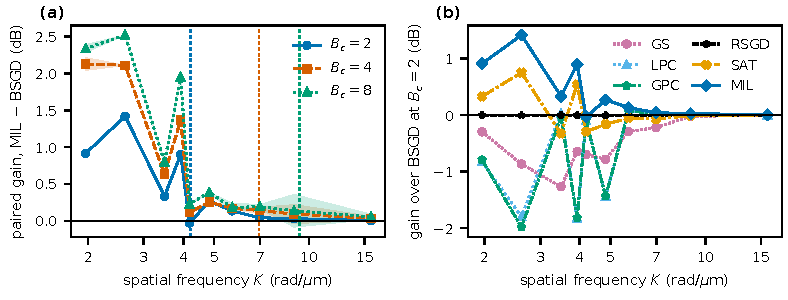
\includegraphics[width=\linewidth]{../code/figures/paper/Fig1_paired_gain.pdf}
\caption{(a) Paired gain (MIL $-$ BSGD) versus spatial frequency for three
contrast budgets; shading, 95\% $t$-intervals over three seeds; dashed lines,
heuristic $K_c(B_c)$. (b) Gain of every non-oracle method over BSGD at
$B_c=2$ (seed means); RSGD coincides with BSGD.}
\label{fig:gain}
\end{figure}

Figure~\ref{fig:recon} shows single-seed reconstructions at the three $K$ of
the ablation studies; Supplement 1, Fig.~S1, shows the corresponding exposures
and index profiles. At the lowest $K$ MIL recovers most of the bar contrast
that BSGD loses; at the highest, both reconstructions are similarly shallow.

\begin{figure}[!htbp]
\centering
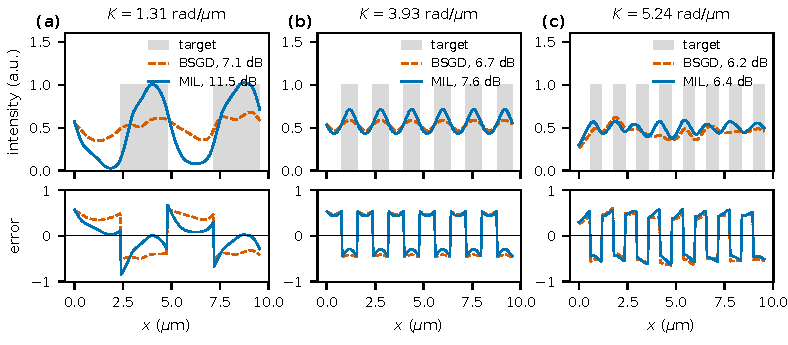
\includegraphics[width=\linewidth]{../code/figures/paper/Fig2_reconstructions.pdf}
\caption{Target, BSGD and MIL reconstructions (top) and errors (bottom) at
$B_c=2$, seed \ROneSeedValue, over a $9.6\,\mu$m section of the window;
legends give $\mathrm{PSNR}_{\text{si}}$. Single-seed illustrations;
Fig.~\ref{fig:gain} carries the statistics.}
\label{fig:recon}
\end{figure}

\subsection{Failure rate against an oracle reference}
\label{sec:failure-rate}
Each exposure of a write-once medium consumes material, so we also count how
often a method falls far short of what is achievable: an exposure fails if its
PSNR is more than a threshold below the constrained oracle's in the same cell
(Table~\ref{tab:failure-rate}; the \WastedMediaThreshDB\,dB threshold was fixed
before the results were computed). At \WastedMediaThreshDB\,dB,
\WastedMediaBSGDFrac\% of BSGD cells and \WastedMediaMILFrac\% of MIL cells
fail, and at \param{3}\,dB \WastedMediaBSGDFracThreeDB\% and
\WastedMediaMILFracThreeDB\%; at \param{1}\,dB the rates are similar (\WastedMediaBSGDFracOneDB\% and \WastedMediaMILFracOneDB\%).
MIL removes the large shortfalls, not the small ones. The rates are relative to
a numerical reference over \WastedMediaNConfigs{} cells, not to a proven
optimum or over physical trials.

\begin{table}[!htbp]
\centering
\caption{Failure rate: percentage of the \WastedMediaNConfigs{} grid cells in
which a method's seed-mean PSNR is more than the column threshold below the
constrained oracle's.}
\label{tab:failure-rate}
\begin{tabular}{lccccccc}
\hline
Threshold & GS & LPC & GPC & BSGD & RSGD & SAT & MIL \\
\hline
\param{1}\,dB & \WastedMediaGSFracOneDB & \WastedMediaLPCFracOneDB & \WastedMediaGPCFracOneDB & \WastedMediaBSGDFracOneDB & \WastedMediaRSGDFracOneDB & \WastedMediaSATFracOneDB & \WastedMediaMILFracOneDB \\
\WastedMediaThreshDB\,dB & \WastedMediaGSFrac & \WastedMediaLPCFrac & \WastedMediaGPCFrac & \WastedMediaBSGDFrac & \WastedMediaRSGDFrac & \WastedMediaSATFrac & \WastedMediaMILFrac \\
\param{3}\,dB & \WastedMediaGSFracThreeDB & \WastedMediaLPCFracThreeDB & \WastedMediaGPCFracThreeDB & \WastedMediaBSGDFracThreeDB & \WastedMediaRSGDFracThreeDB & \WastedMediaSATFracThreeDB & \WastedMediaMILFracThreeDB \\
\hline
\end{tabular}
\end{table}

\subsection{Other baselines and the saturation-only surrogate}
\label{sec:baselines}
At $B_c=2$ (Fig.~\ref{fig:gain}(b)), GS (\GSGainMin{} to \GSGainMax\,dB)
never improves on BSGD and LPC (\LPCGainMin{} to \LPCGainMax\,dB) improves on
it by at most \LPCGainMax\,dB; GPC (\GPCGainMin{} to \GPCGainMax\,dB) differs
from LPC by at most \GPCLPCMaxAbsDiffTwoX\,dB, consistent with both hitting
the same contrast clip. LPC is the closed-form use of the heuristic transfer
function, so its failure is further evidence that the small-signal picture does
not describe this regime. The saturation-only surrogate tests whether transport
needs to be modelled at all: averaged over $K$, its gain is
\SATFracOfMILTwoX\%, \SATFracOfMILFourX\% and \SATFracOfMILEightX\% of MIL's at
$B_c=2$, 4 and 8, and by cell it recovers
\SATFracLowKMin--\SATFracLowKMax\% of MIL's gain at $K=1.96$\,rad/\textmu m and
\SATFracSecondKMin--\SATFracSecondKMax\% at $K=2.62$\,rad/\textmu m but scores
below BSGD in \SATNBelowBSGD{} of the \SATNCells{} cells where the ratio is
defined. A pointwise surrogate is therefore useful only at the lowest spatial
frequencies; elsewhere the full recording model is needed for any gain.

\subsection{Compute-matched control}
\label{sec:compute-matched}
MIL's per-iteration cost is about \ComputeMatchRatio$\times$ that of BSGD (one
wall-clock measurement). With \ComputeMatchRatio$\times$ more BSGD iterations
at the three ablation $K$ (Supplement 1, Section S6) the paired gain is
\MTwoRGainSub, \MTwoRGainNear{} and \MTwoRGainPost\,dB at $K=\SOneKSub$,
\SOneKNear{} and \SOneKPost\,rad/\textmu m, against \SOneGBaselineSub,
\SOneGBaselineNear{} and \SOneGBaselinePost\,dB at equal iteration count: the
extra iterations narrow the gap at the two lower $K$ but it stays positive at
all three. Wall-clock time is a noisy proxy for compute, so this tests a much
larger baseline budget rather than an equal-FLOP comparison.

\subsection{Which recording nonlinearity produces the gain}
\label{sec:mechanism}
Removing one mechanism at a time (Table~\ref{tab:mechanism}, top) leaves a
positive gain at every $K$, and which removal matters depends on $K$:
linearizing the index map raises the gain at $K=\SOneKSub$ and \SOneKPost{}
but lowers it at \SOneKNear\,rad/\textmu m. Because three mechanisms saturate
the dose response, removing one leaves the others, so we also ran all $2^3$
on/off combinations of monomer depletion (removed by holding $u=1$), dye
bleaching ($k_{\text{bleach}}=0$) and the $\tanh$ map (Supplement 1,
Section S2). Removing monomer depletion at fixed $\kappa$ raises the polymer
cured by unit dose from $N\approx1$ to $N\approx8.7$, so these conditions are
run with $\kappa$ rescaled to restore $N(E{=}1)=1$. A final control removes all
three and sets $\kappa=1/(1.5\,t_{\text{total}})$, which makes the recording
BSGD's own linear model up to non-local blur and shrinkage. The factorial ran on
CPU and reproduces the GPU full-model values to within \SXDeviceMaxDiff\,dB.

\begin{table}[!htbp]
\centering
\caption{Paired gain (dB) under mechanism ablations, $B_c=2$, mean of three
seeds. Top: one mechanism removed. Bottom: saturating mechanisms isolated at a
matched operating point, $N(E{=}1)=1$, and the slope-matched linear control;
blur, diffusion and shrinkage are kept. Intervals: Supplement 1, Figs.~S2--S3.}
\label{tab:mechanism}
\small\renewcommand{\arraystretch}{1.2}
\begin{tabular}{lccc}
\hline
Condition & $K=\SOneKSub$ & $K=\SOneKNear$ & $K=\SOneKPost$ \\
\hline
Full model & \SOneGBaselineSub & \SOneGBaselineNear & \SOneGBaselinePost \\
No non-locality ($\sigma=0$) & \SOneGNoNonlocSub & \SOneGNoNonlocNear & \SOneGNoNonlocPost \\
No diffusion ($D_0=0$) & \SOneGNoDiffSub & \SOneGNoDiffNear & \SOneGNoDiffPost \\
No dye bleaching ($k_{\text{bleach}}=0$) & \SOneGNoDyeSub & \SOneGNoDyeNear & \SOneGNoDyePost \\
No index saturation ($\tanh$ linearized) & \SOneGNoSatSub & \SOneGNoSatNear & \SOneGNoSatPost \\
\hline
Only monomer depletion & \SXGOnlyMonomerSub & \SXGOnlyMonomerNear & \SXGOnlyMonomerPost \\
Only dye bleaching & \SXGOnlyDyeMatchedSub & \SXGOnlyDyeMatchedNear & \SXGOnlyDyeMatchedPost \\
Only $\tanh$ map & \SXGOnlyTanhMatchedSub & \SXGOnlyTanhMatchedNear & \SXGOnlyTanhMatchedPost \\
Dye bleaching and $\tanh$ map & \SXGNoMonomerMatchedSub & \SXGNoMonomerMatchedNear & \SXGNoMonomerMatchedPost \\
Linear, slope-matched & \SXGLinearMatchedSub & \SXGLinearMatchedNear & \SXGLinearMatchedPost \\
\hline
\end{tabular}
\end{table}

Three observations follow. First, when the recording is the media-blind model
up to blur and shrinkage, MIL gains essentially nothing at the two lower $K$, so
the gain there requires a nonlinear dose response; at $K=\SOneKPost$\,rad/\textmu m
the linear control's gain (\SXGLinearMatchedPost\,dB) is comparable to the full
model's (\SOneGBaselinePost\,dB), so the small gain there may come from the blur
and shrinkage that BSGD ignores. Second, each saturating mechanism alone
produces a gain at the two lower $K$, so no single mechanism is necessary.
Third, monomer depletion alone gives a larger gain than the full model at every
$K$, so the mechanisms' effects do not add. In this model, then, the low-$K$
gain comes from designing through whichever dose-response nonlinearity is
present. The matching criterion $N(E{=}1)=1$ is our choice; another
normalization could reorder the single mechanisms, though not the null result of
the linear control. Unmatched conditions are discussed in Supplement 1,
Section S2.

\subsection{Dependence on grating slant}
\label{sec:slant}
With everything else fixed, the paired gain depends strongly and
non-monotonically on the fringe slant $\phi$ (Fig.~\ref{fig:slant}(a);
Supplement 1, Section S3). At $\phi=0^\circ$, $5^\circ$, $10^\circ$ and
$20^\circ$ it is \SEightGainKLowSlantZero, \SEightGainKLowSlantFive,
\SEightGainKLowSlantTen{} and \SEightGainKLowSlantTwenty\,dB at
$K=1.96$\,rad/\textmu m and \SEightGainKMidSlantZero,
\SEightGainKMidSlantFive, \SEightGainKMidSlantTen{} and
\SEightGainKMidSlantTwenty\,dB at $K=\SOneKNear$\,rad/\textmu m: small slants
increase the gain and larger ones remove most of it. The scalar readout
disagrees with RCWA for slanted gratings (Section~\ref{sec:discussion}), so
these values are model-dependent; this is why the headline results are
restricted to unslanted gratings and should not be read as predictions for
slanted holograms.

\begin{figure}[!htbp]
\centering
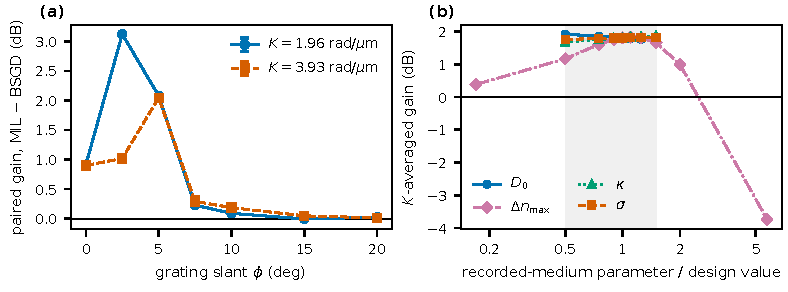
\includegraphics[width=\linewidth]{../code/figures/paper/Fig3_slant_mismatch.pdf}
\caption{(a) Paired gain versus grating slant, $B_c=2$, 95\% $t$-intervals
over three seeds. (b) Gain when both exposures are designed with nominal
parameters and recorded on a twin with one parameter scaled, averaged over the
three ablation $K$ ($B_c=2$; shading, 95\% intervals; grey band, $\pm50\%$).}
\label{fig:slant}
\end{figure}

\subsection{Robustness to twin miscalibration}
\label{sec:robustness}
\textbf{One parameter.} Here both exposures are designed once with the nominal
parameters and recorded, without re-optimization, on a twin with $D_0$,
$\sigma$, $\kappa$ or $\Delta n_{\max}$ perturbed by $\pm10$, $\pm25$ or
$\pm50\%$ (Fig.~\ref{fig:slant}(b); Supplement 1, Section S4). BSGD's design
uses no recording parameter (only $\Delta n_{\max}$, as the scale of its linear
model), so the test measures how much MIL's advantage depends on a correct
twin. The $K$-averaged gain ranges from \SThreeWorstWithinFifty{} to
\SThreeBestWithinFifty\,dB (nominal \SThreeNominalGain\,dB). We swept
$\Delta n_{\max}$ further because two fits of the twin to Bayfol HX data
disagree on it by \BayfolDnMaxRatio$\times$ (Section~\ref{sec:twin-validation}):
the gain is \SThreeDnMaxAtMostNegative\,dB at
$\SThreeDnMaxMostNegativePct\%$, \SThreeDnMaxAtPlusFifty\,dB at $+50\%$,
\SThreeDnMaxAtHundred\,dB at $+100\%$ and \SThreeDnMaxAtMostPositive\,dB at
$+\SThreeDnMaxMostPositivePct\%$. A twin that underestimates the medium's
index budget several-fold can therefore make MIL worse than the media-blind
baseline; where between $+100\%$ and $+\SThreeDnMaxMostPositivePct\%$ the sign
changes was not resolved.

\textbf{Joint and structural errors.} In \SSixNDraws{} Monte Carlo draws with
all four parameters perturbed independently and uniformly within
$\pm$\SSixPctRange\% (same designed exposures), the $K$-averaged gain ranges from
\SSixWorstDrawGain{} to \SSixBestDrawGain\,dB (mean \SSixMeanGain\,dB,
bootstrap 95\% interval [\SSixBootCILo, \SSixBootCIHi]); \SSixNNegative{} of
\SSixNDraws{} are negative. Beer--Lambert attenuation through depth (16 recorded
slices) gives \SSevenGainODZero, \SSevenGainODOneTenth{} and
\SSevenGainODThreeTenths\,dB at optical density 0, 0.1 and 0.3. Re-optimizing
both arms on media with $D_0$, $\sigma$ or $\kappa$ changed by up to $\pm50\%$
($K=\SOneKPost$\,rad/\textmu m) gives \STwoGainMin{} to \STwoGainMax\,dB
(nominal \STwoBaselineGain\,dB).

\textbf{Targets and noise.} At $K=\SOneKNear$\,rad/\textmu m and $B_c=2$ the
gain is \SFourGainBarsTwoX{} for bars, \SFourGainSpotsTwoX{} for sparse random
spots and \SFourGainRandomBinaryTwoX\,dB for a random binary target, and
Gaussian detector noise at \SFiveNoiseStdPct\% of the peak changes the bar
gain from \SFiveNoiselessGain{} to \SFiveNoisyGain\,dB (Supplement 1,
Section S8).

\section{Twin validation against published data}
\label{sec:twin-validation}
We fit the twin to the first-harmonic index modulation $\Delta n_1$ versus
dose in Fig.~3 of Bruder et al.~\cite{bruder2017bayfol} (Bayfol HX,
$\Lambda=700$\,nm, $K=8.98$\,rad/\textmu m): the source's kinetic-model curve
(16.7\,mW/cm$^2$) and its measurement (19.2\,mW/cm$^2$), read visually rather
than with a calibrated digitizer (about $\pm10\%$ in dose, $\pm3$--$5\%$ in
$\Delta n_1$). Unfitted parameters take Bayfol HX values from the released
configuration; each fit is the best of 8--10 random starts, and NRMSE is the
root-mean-square residual over the range of the fitted data.

\textbf{Fits and held-out prediction.} With $\kappa$, $\Delta n_{\max}$ and
$k_{\text{bleach}}$ free, the twin reproduces the rise-then-decline shape of
both series (Fig.~\ref{fig:twin}; in-sample NRMSE \HoldoutBSimIn{} for the
model curve, \HoldoutBExpIn{} for the measurement). Both are plotted against
dose and the twin is dose-reciprocal at $\gamma=1$, so a fit to one series
predicts the other without refitting, with NRMSE \HoldoutBSimOut{} (model to
measurement) and \HoldoutBExpOut{} (the reverse). The fitted
$k_{\text{bleach}}$ are \HoldoutBSimKbleach{} and \HoldoutBExpKbleach{} (default
0.2) and the fitted $\Delta n_{\max}$ \HoldoutBSimDnMax{} and
\HoldoutBExpDnMax. With $k_{\text{bleach}}$ held at 0.2 the in-sample NRMSE is
\NRMSEBruderGrowthDnKSim{} and \NRMSEBruderGrowthDnKExp, but the measured-series
optimum is degenerate (its $\kappa$ saturates the medium before the first
measured dose, giving an almost constant $\Delta n_1$; Supplement 1, Fig.~S5),
the held-out NRMSEs are \HoldoutASimOut{} and \HoldoutAExpOut, and the fitted
$\Delta n_{\max}$ disagree by \BayfolDnMaxRatio$\times$, which sets the range of
the $\Delta n_{\max}$ sweep in Section~\ref{sec:robustness}. Fig.~S5 also shows
a fit to a PQ/PMMA $\Delta n_1(t)$ model curve~\cite{hsieh2022pqpmma} outside
the tested $K$ range (NRMSE \NRMSEHsiehGrowthDnK).

\begin{figure}[!htbp]
\centering
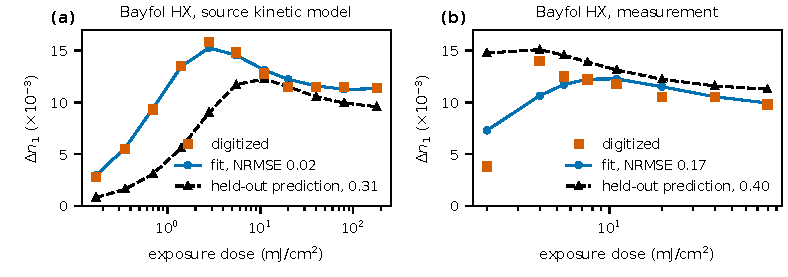
\includegraphics[width=\linewidth]{../code/figures/paper/Fig4_twin_validation.pdf}
\caption{Twin fitted to $\Delta n_1$ digitized from Bruder et
al.~\cite{bruder2017bayfol} (Bayfol HX): (a) the source's kinetic-model curve,
(b) its measurement. Solid, fit to the series shown ($\kappa$,
$\Delta n_{\max}$, $k_{\text{bleach}}$ free); dashed, parameter-free
prediction from the fit to the other series. Legends give NRMSE.}
\label{fig:twin}
\end{figure}

\textbf{What this establishes.} The model family can reproduce, and predict
across two views of the same condition, the dose response of one commercial
photopolymer with effective parameters. It does not pin the default medium of
Table~\ref{tab:mediumparams} to a real material or test transfer across $K$ or
media: the two series share a material, a grating and nearly the same
intensity, and one is a model output. $D_0$ and $\sigma$ are identifiable only
from multi-$K$ growth-curve families, which we did not have. The headline
claims therefore rest on the paired design and the miscalibration tests, not on
absolute agreement with a real medium.

\section{Discussion and limitations}
\label{sec:discussion}
\textbf{Scope.} All results are simulation outputs of one model family for
one-dimensional transverse recording of binary bar targets in unslanted
gratings, with one default medium and three seeds per cell. Whether the gains
transfer to a physical photopolymer is untested; the decisive experiment,
recording optimized and media-blind exposures in a characterized medium and
comparing the measured reconstructions, is future work.

\textbf{Readout validity.} Against RCWA~\cite{moharam1981rigorous} (computed
with TORCWA~\cite{kim2023torcwa}) over a \RCWAVGridNCases-case grid of $K$,
$\Delta n$, polarization and slant, Kogelnik theory deviates by at most
\RCWAUnslantedMaxDev{} in diffraction efficiency for unslanted geometries but
by up to \RCWAVGridMaxDev{} at a $20^\circ$ slant (Supplement 1, Section S5).
The check concerns the closed-form reference, but the beam propagation in the
design loop shares its paraxial scalar approximation, so validated claims are
restricted to unslanted gratings, a restriction that matters
(Section~\ref{sec:slant}).

\textbf{Model and statistics.} The recorded profile is uniform through depth
except in the Beer--Lambert check; diffusion uses a spatially averaged
coefficient; the index map and its shape constant are modelling choices;
shrinkage is a placeholder; the medium parameters are illustrative; and the
factorial covers interactions among the saturating mechanisms only. Three
seeds per cell measure initialization sensitivity, which is small here; model
and parameter error are probed only by the miscalibration studies over the
stated ranges. The \MOneNK-point grid does not resolve features between grid
points, such as the zero crossing at $B_c=2$.

\textbf{Implications for practice.} If the twin's qualitative response is
right, exposure-domain optimization through a recording model is most useful
at low spatial frequency and in unslanted geometry, and its main benefit is
removing large shortfalls (Table~\ref{tab:failure-rate}) rather than raising
average quality. Calibrating the twin for a new medium needs $\kappa$ and
$\Delta n_{\max}$ from a dose-response curve measured under the same
condition, $D_0$ and $\sigma$ from several spatial frequencies, and a fitted
dye-bleaching rate (Supplement 1, Section S7); a several-fold underestimate of
$\Delta n_{\max}$ is the error most likely to reverse the benefit.

\section{Conclusion}
\label{sec:conclusion}
In simulation, designing the exposure of a write-once volume photopolymer
through a differentiable NPDD and beam-propagation model improves on
media-blind design in \MOneNPositive{} of \MOneNCells{} unslanted grating
cells, by up to \MaxGainEightX\,dB at low spatial frequency, and removes the
exposures that fall more than \WastedMediaThreshDB\,dB short of an oracle
reference. The gain requires a nonlinear dose response but no single saturating
mechanism, decays toward zero at high spatial frequency and under fringe slant,
survives joint parameter errors of $\pm$\SSixPctRange\%, and can reverse if the
twin underestimates the index budget several-fold. Testing these model
predictions in a recorded medium is the next step.

\begin{backmatter}

\bmsection{Funding}
This research received no external funding.

\bmsection{Acknowledgment}
The author used Claude (Anthropic; Claude Code with the Claude Sonnet 5 and
Claude Opus 4.8, 5 and 5.5 models) to write and debug simulation and analysis
code, to read the data points digitized in Section~\ref{sec:twin-validation},
and to draft and edit the text; the author reviewed all outputs and takes full
responsibility for the content.

\bmsection{Disclosures}
The author declares no conflicts of interest.

\bmsection{Data availability}
Code, experiment manifests, raw per-job result files and the scripts that
generate every number and figure in this paper are available on GitHub
(\url{https://github.com/ultramagnus23/HoloForge}) and archived in
Ref.~\cite{holoforge2026code}.

\bmsection{Supplemental document}
See Supplement 1 for supporting content.

\end{backmatter}

\bibliography{refs}

\end{document}
